% Conversion avec : convert -density 300 -flatten img.pdf img.png
\documentclass{standalone}
\usepackage{xcolor,pgf,tikz,tkz-tab,pgfplots,xfp}
\pgfplotsset{compat=1.15}
\usetikzlibrary{arrows,backgrounds,calc}
\usepackage{esvect}
\renewcommand{\vec}{\vv}
\begin{document}

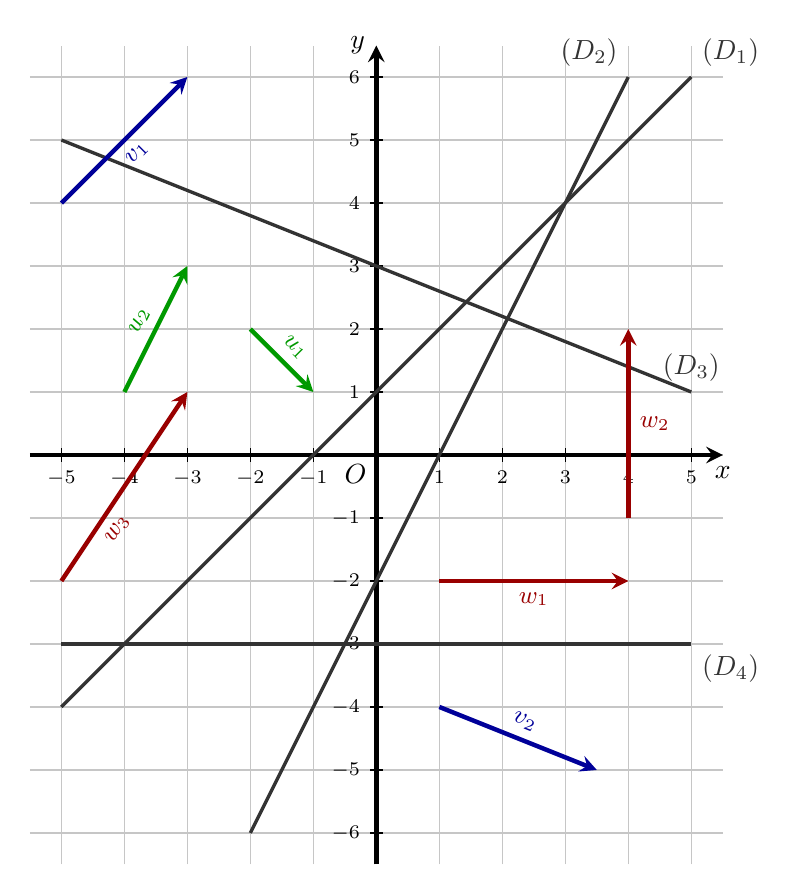
\begin{tikzpicture}[scale=0.8, >=stealth]

	% ==========================================
	% 1. LE CADRE ET LA GRILLE (Seyès style)
	% ==========================================
	% Grille fine (petits carreaux)
	\draw[help lines, color=gray!45, thin] (-5.5,-6.5) grid (5.5,6.5);
	% Grille principale (unités)
	% \draw[help lines, color=gray!40, thick] (-5,-6) grid (5,6);

	% Axes
	\draw[->, ultra thick] (-5.5,0) -- (5.5,0) node[below] {$x$};
	\draw[->, ultra thick] (0,-6.5) -- (0,6.5) node[left] {$y$};

	% Graduation complète
	\foreach \x in {-5,-4,...,-1,1,2,...,5}
	\draw (\x,3pt) -- (\x,-3pt) node[below, font=\scriptsize] {$\x$};
	\foreach \y in {-6,-5,...,-1,1,2,...,6}
	\draw (3pt,\y) -- (-3pt,\y) node[left, font=\scriptsize] {$\y$};
	\node[below left, font=\bfseries] at (0,0) {$O$};


	% ==========================================
	% 2. LES DROITES CROISSANTES (Bleues)
	% ==========================================
	% D1 : y = x + 1 (Pente 1)
	\draw[black!80!white, very thick] (-5,-4) -- (5,6) node[above right] {$(D_1)$};

	% D2 : y = 2x - 2 (Pente 2, plus pentue)
	\draw[black!80!white, very thick] (-2,-6) -- (4,6) node[above left] {$(D_2)$};

	% D3 : y = 0.5x + 3 (Pente 0.5, peu pentue)
	\draw[black!80!white, very thick] (-5,5) -- (5,1) node[above] {$(D_3)$};

	% Dh : y = -3 (Pente 0, horizontale - PIÈGE)
	\draw[black!80!white, very thick] (-5,-3) -- (5,-3) node[below right] {$(D_4)$};


	% ==========================================
	% 3. LES VECTEURS (Le Bazar !)
	% ==========================================

	% --- A. VECTEURS DIRECTEURS "FACILES" (En Vert, sur la droite) ---
	% u1 pour D1 : (1,1) dessiné à partir de (-2,-1)
	\draw[->, green!60!black, ultra thick] (-2,2) -- +(1,-1) node[midway, sloped, above, font=\small] {$\vec{u_1}$};
	\draw[->, green!60!black, ultra thick] (1-5,1) -- (2-5,3) node[midway, sloped, above, font=\small] {$\vec{u_2}$};


	% --- B. VECTEURS DIRECTEURS "LOIN" (En Orange, colinéaires mais ailleurs) ---
	% v1 pour D1 : (2,2) dessiné en haut à gauche
	\draw[->, blue!60!black, ultra thick] (-5,4) -- (-3,6) node[midway, sloped, below, font=\small] {$\vec{v_1}$};
	\draw[->, blue!60!black, ultra thick] (1,-4) -- +(2.5,-1) node[midway, sloped, above, font=\small] {$\vec{v_2}$};


	% --- C. VECTEURS NON-DIRECTEURS (En Rouge, "servent à rien") ---
	\draw[->, red!60!black, ultra thick] (1,-2) -- (4,-2) node[midway, below, font=\small] {$\vec{w_1}$};
	\draw[->, red!60!black, ultra thick] (4,-1) -- (4,2) node[midway, right, font=\small] {$\vec{w_2}$};
	\draw[->, red!60!black, ultra thick] (-5,-2) -- (-3,1) node[midway, sloped, below, xshift=-5mm, font=\small] {$\vec{w_3}$};

\end{tikzpicture}

\end{document}
